\chapter{Progettazione concettuale}
    \section{Introduzione}
        \fontsize{15}{14}\selectfont{ In questa sezione verrà introdotta la progettazione concettuale dell'applicativo. Partendo da un primo diagramma di classe in UML. Dal risultato dell'analisi dei requisiti che devono essere soddisfatti si arriverà a uno schema concettuale ristrutturato. Saranno evidenziati i concetti rilevanti ai fini della rappresentazione dei dati e le relazioni che intercorrono tra di esse.}
        
\section{Class Diagram}
    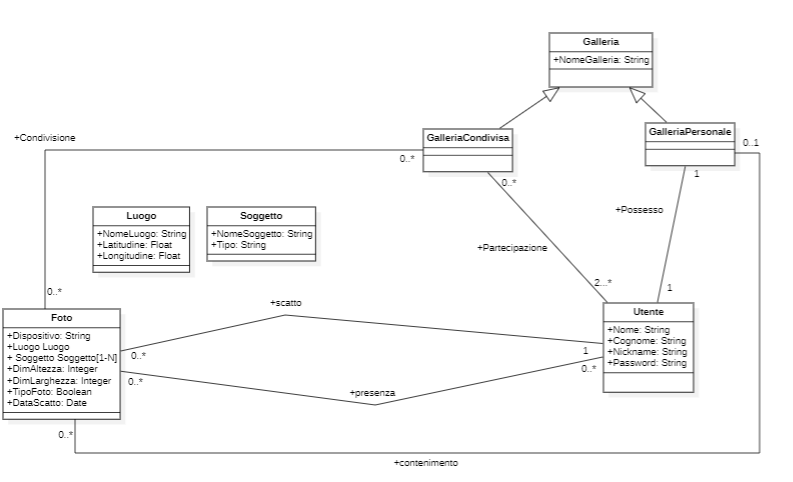
\includegraphics{immagini/MC.png}
        
    \section{Analisi della ristrutturazione del Class Diagram}
        
        \subsection{Analisi delle ridondanze}
            Assenza di ridondanze all'interno del DB
            
        \subsection{Analisi degli identificativi Primari}
            Identificativo dell’entità Utente: Nickname
            \newline
            Inserito un codice identificativo per l’entità foto: CodFoto
            \newline
            Identificativo dell’entità Luogo: NomeLuogo
            \newline
            Inserito un codice identificativo per l’entità soggetto: CodSoggetto
             \newline
            Inserito un codice identificativo della Galleria, ereditato dall’entità 
            figlia GalleriaCondivisa: CodGP
             \newline
            Inserito un codice identificativo della Galleria, ereditato dall’entità figlia GalleriaCondivisa: CodGC
             \newline
        \subsection{Rimozione degli attributi multipli}
            L’attributo Soggetto è stato separato dall’entità di appartenenza Foto e messo in relazione con essa tramite una relazione molti a molti
        \subsection{Rimozione degli attributi composti}
            Gli attributi Luogo e Soggetto sono stati separati dall’entità Foto, andando a formare due nuove entità
        \subsection{Partizione/Accorpamento delle associazioni}
            Non vi sono partizionamenti o accorpamenti delle associazioni
        \subsection{Rimozione delle gerarchie}
        L’entità padre Galleria è stata rimossa e i suoi attributi sono stati ereditati dalle entità figlie Galleria Personale e Galleria Condivisa
\section{Class Diagram ristrutturato}
    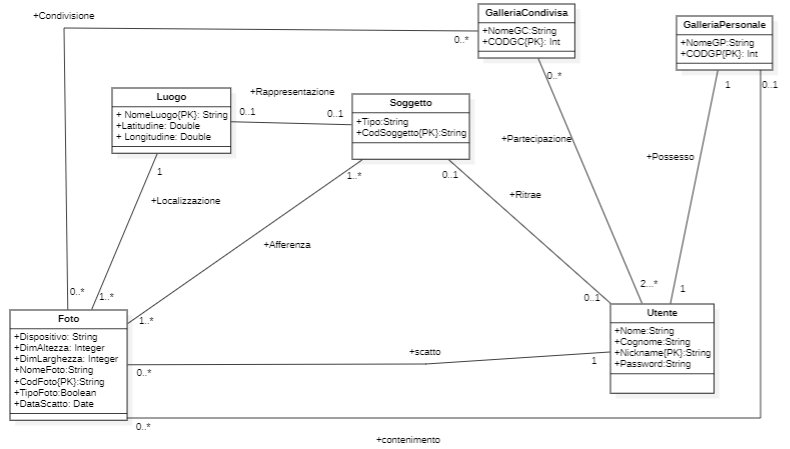
\includegraphics{immagini/MCR.png}

\section{Class Diagram ristrutturato in ER}
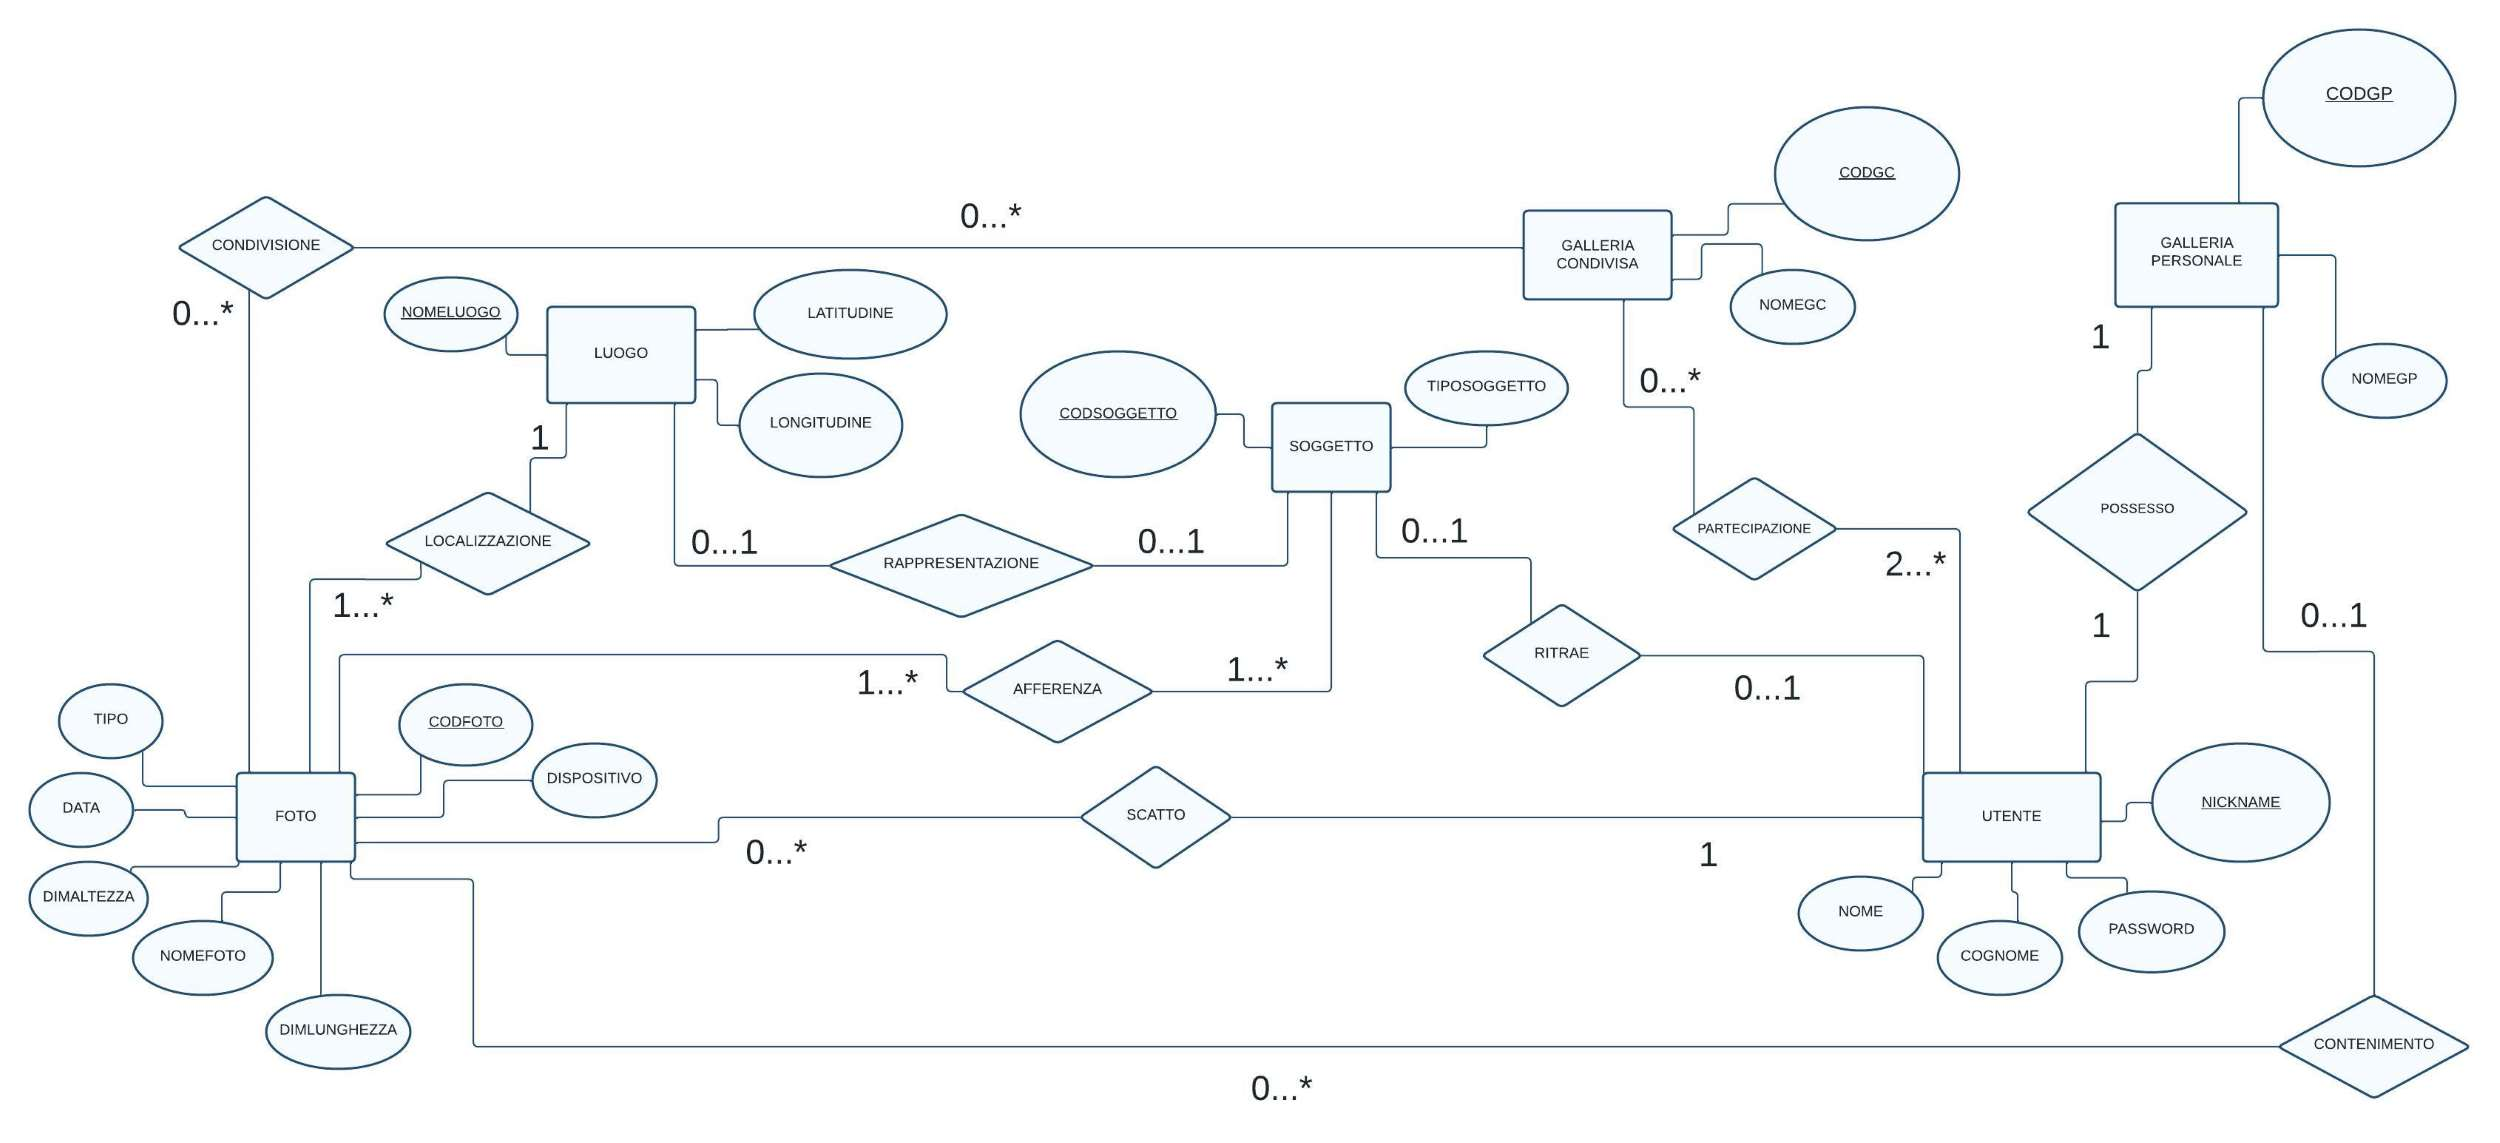
\includegraphics[width=1.4\textwidth]{immagini/Galleria Fotografica Geocalizzata .jpg}